% !TEX encoding = UTF-8 Unicode
\documentclass[fleqn,twoside]{article}
\usepackage[ngerman]{babel}
\usepackage[utf8]{inputenc}
\usepackage[T1]{fontenc}
\usepackage{graphicx}
\usepackage{fancyhdr}
\usepackage{amssymb}
\usepackage{amsmath}
\usepackage{cite}
\usepackage{eurosym}
\usepackage{wrapfig}
\usepackage{tabularx}
\usepackage{pdfpages}
\usepackage{nicefrac}
\usepackage{wasysym}
\usepackage{multirow}
\usepackage{pifont}
\usepackage{textcomp}
\usepackage{comment}
%\usepackage{units}
\usepackage{siunitx}
\usepackage{yfonts}
\usepackage{calligra}
\usepackage{csquotes}
%\usepackage{emerald}
\usepackage{titlesec}
\usepackage{tikz}
\usepackage{stanli}
\usepackage{romanbar}
\usepackage{graphicx}
\usepackage{tabto}
\usepackage{todonotes}
%\usepackage{3dstructuralanalysis}
%\usepackage{structuralanalysis}
\usepackage{enumitem}
\usepackage{booktabs}
\usepackage{float}


%Befehle abändern
%Itemize ohne Lücken
\setlist[itemize]{noitemsep, topsep=2pt}
\raggedbottom
%\renewcommand{\todo}[1]{\todo[inline]{#1}}


%Betragsfunktion
\newcommand{\abs}[1]{\ensuremath{\left\vert#1\right\vert}}
%Einheitenfunktion
\newcommand{\un}[2]{{\unit[#1]{\color{black!100}[#2]}}}

\usepackage[pdftex, colorlinks, linkcolor=black, frenchlinks]{hyperref}
\usepackage[a4paper , lmargin = {2.5cm} , rmargin = {2cm} , tmargin = {2.5cm} , bmargin = {2.5cm} ]{geometry}
\pagestyle{fancy}

\title{\Huge{\textfrak{Kontinumsmechanik}}}
\author{\calligra{Jonas Konrad}}
\date{\textfrak{\today}}

\begin{document}
\parindent 0pt
\fancyhead[L]{Jonas Konrad}
\fancyfoot[L]{\frakfamily J. K.}
\fancyfoot[R]{\frakfamily }
\fancyfoot[C]{\frakfamily Die Lehre der Kartoffel\\Seite \thepage}
\maketitle \thispagestyle{empty}
%\initfamily %Für Initialien
\begin{center}
\textfrak{Diese Formelsammlung wurde im Sommersemester 2022 von Jonas Konrad verfasst.\\Dozent: Dr.-Ing. Marlon Franke , Übungsleiter: M.Sc. Timo Ströhle\\Kein Anspruch auf Vollständigkeit oder Fehlerfreiheit.\\LaTex Vorlage liegt Fachschaft vor}
\end{center}
\tableofcontents
%\listoftodos
\newpage

\section{Grundbegriffe}
\begin{itemize}
    \item istotroper Tensor: richtungsunabhängiger Tensor
    \item Rotation: $\det(A)=1$
    \item Reflexion/Spiegelung: $\det(A)=-1$
\end{itemize}


\section{Tensoren}

\subsection{Invarianten}
\begin{itemize}
    \item Invarianten einer 3x3 Matrix (A):
        \begin{tabular}{c|c|c}
            I & spur(A) & $\lambda_1 + \lambda_2 + \lambda_3$ \\
            II & $\frac12 (spur(A)^2-spur(A^2))$ & $\lambda_1\lambda_2+\lambda_2\lambda_3+\lambda_3\lambda_1$ \\
            III & det(A) & $\lambda_1\lambda_2\lambda_3$
        \end{tabular}
    \item Hauptinvarianten des rechten Cauchy-Green Tensors: \\Maße für Änderung der Linien-, Flächen und Volumenelemente
\end{itemize}
\subsection{Kreuzprodukt}
\begin{itemize}
    \item Kreuzprodukt in Indexschreibweise
        \[ a\times b = \varepsilon_{ijk} \underline{e}_i a_j b_k = \begin{array}{c}  \phantom{+}(a_2b_3-a_3b_2)\underline{e}_1\\
                                                                                                +(a_3b_1-a_1b_3)\underline{e}_2\\
                                                                                                +(a_1b_2-a_2b_1)\underline{e}_3\\
                                                                                                \end{array}  \]
    \item Spatprodukt in Indexschreibweise: $a_i \cdot (b \times c) = \varepsilon_{ijk} a_i b_j c_k$
\end{itemize}
\subsection{Permutationssymbol}
\begin{itemize}
	\item Permutationssymbol :
			\[ \varepsilon_{ijk} =
			\begin{tabular}{c l} 
			1 & für alle geraden Permutationen von ijk {z.B.:} $\varepsilon_{231}, \varepsilon_{123}, \varepsilon_{312}...$\\ 
			-1 & für ungerade Permutationen z.B.: $\varepsilon_{321}, \varepsilon_{213}...$\\  
			0 & für $\geq 2$ Indizes gleich  
			\end{tabular}  	\]
\end{itemize}
\subsection{Kroneckerdelta}
\begin{itemize}
	\item Kroneckerdelta:
			\[ \delta_{ij}=\underline{e}_i \cdot \underline{e}_j=\begin{tabular}{c c l} 1 & für & $\underline{e}_i=\underline{e}_j$ \\ 0 & für &  $\underline{e}_i \neq \underline{e}_j$ \end{tabular} 	\]
\end{itemize}

\subsection{Weitere Operationen}
\begin{itemize}
	 \item Rotation-polare Zerlegung: $F=R\cdot U = v\cdot R$\\ 
	 $\Rightarrow$ Zerlegung von Deformation in Rotation und reine Streckung; U \& v sym. und positiv definit
	 \item Aufteilung Tensor (2.) Stufe in symmetrischen ($\underline{A}=\underline{A}^T$) und schief/antimetrischen Anteil ($\underline{A}=-\underline{A}^T$):\\
	 $A=A^{sym}+A^{skw} = \frac12 \cdot (A+A^T) + \frac12 (A-A^T)$
	 \item Aufteilung Tensor (2.) Stufe in Kugeltensor und deviatorischen Anteil:\\
	 (Meist Spannungstensor) $\sigma=\sigma^{vol}+\sigma^{dev}$ ; $\sigma^{vol}=\frac{\text{spur}(\sigma)}{3}\cdot \underline{I}$ ; $\sigma^{dev} = \sigma-\sigma^{vol}$\\ $\rightarrow \frac{\text{spur}(\sigma)}{3}\overset{\wedge}{=}$ hydrostatischer Druck p
        \item Eigenwert eines Tensors: $\det(\underline{A} - \lambda\underline{I}) \overset{!}{=} 0$
        \item Eigenvektoren: $(\underline{A}-\lambda\underline{I})\cdot n = 0$
        \item Rotationstensor: $R=F\cdot U^{-1}=v^{-1}\cdot F$
        \item Abbildung \enquote{b auf c abbilden}: $c=A\cdot b$
        \item Doppelte Verjüngung: $\underline{A}:\underline{B} = A_{ij}B_{kl}(\overset{\rightarrow}{e_i}\otimes\overset{\rightarrow}{e_j}):(\overset{\rightarrow}{e_k}\otimes\overset{\rightarrow}{e_l}) = A_{ij}B_{kl}(\delta_{ik}):(\delta_{jl}) = A_{kj}B_{kj}$
        \item Gateaux-Differential: $\frac{\delta f(x_0)}{\delta x_i} = \underset{h\rightarrow 0}{\lim} \frac{f(x_{(0,1)},x_{(0,2)},x_{(0,3)},..,x_{(0,n)})}{h} , (i=1,2,3,..,n)$\\ $\Rightarrow$ Mehrdimensionale Ableitung
\end{itemize}

\subsection{Theorieaussagen}
\begin{itemize}
	 \item Aussage des Carly-Hamilton Theorems:\\
	 	Jede quadratische Matrix ist Nullstelle ihres charakteristischen Polynoms (siehe Eigenwertberechnung)
	 \item Bedingung Tensor isochor (volumenerhaltend): $J = \det(A) \overset{!}{=} 1$
	 \item Aussage Cauchy-Theorem: \\
	 Spannungsvektor folgt als lineare Abbildung des Normalenvektors zur willkürlich gewählten Schnittfläche: Vektor: $\overset{\rightarrow}{\sigma}\left(x,\overset{\rightarrow}{n}\right)$; Tensor 2. Stufe: $\underline{\sigma}(x)$
        \item Piola Transformation: Bildet Vektoren zwischen Euler- und Lagrange Koordinaten ab\\
        \begin{minipage}{0.7\textwidth}
            \item Divergenz beschreiben: Quellen und senken eines Tensorfelds um einen Grad
        \end{minipage}
        \begin{minipage}{0.3\textwidth}
                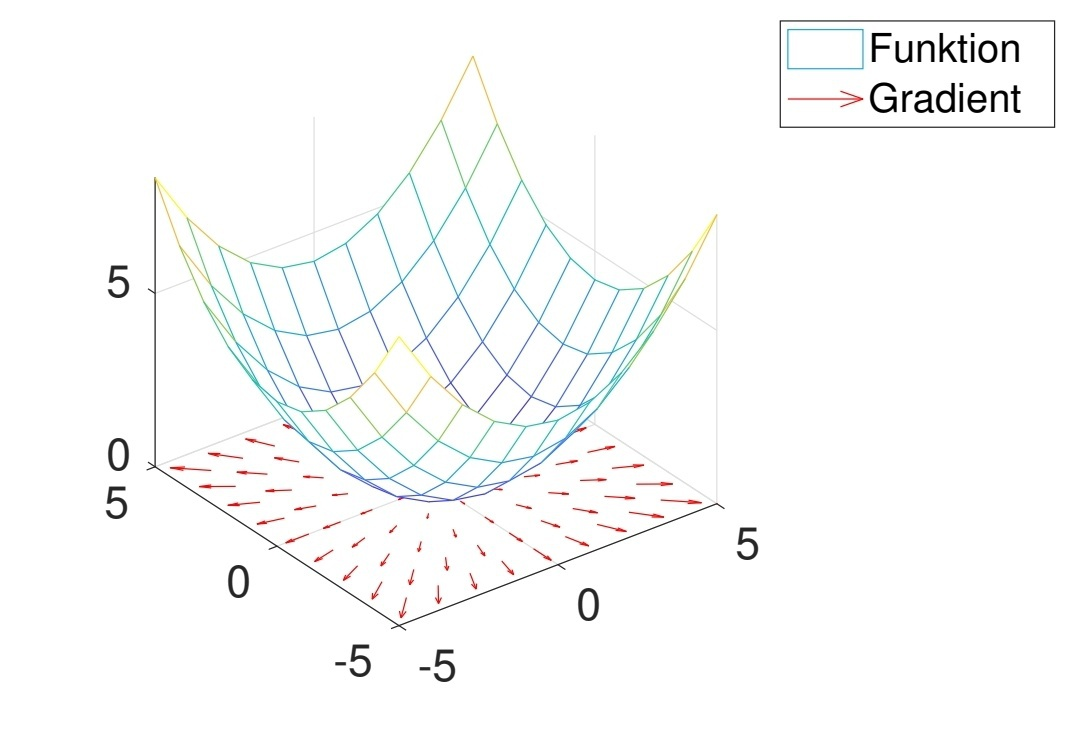
\includegraphics[width=0.99\textwidth]{Grafiken/Quellen_Tensorfeld.jpg}
        \end{minipage}
\end{itemize}

\subsection{Piola-Kirchhoff Spannungstensoren}
    \begin{itemize}
    \item Piola-Kirchhoff Spannungstensor:
	 	\begin{itemize}
	 	  \item 1. PK-Tensor: $P = N^T \overset{\wedge}{=} \frac{\text{aktuelle Kraft}}{\text{Referenzfläche}}$
                \item 2. PK-Tensor: $P= N \cdot F^{T-1}$
	 	\end{itemize}
   \item Bei kleinen Verzerrungen braucht nicht zwischen diesen Spannungstensoren unterschieden zu werden
   \end{itemize}
   
\subsection{Deformations- und Verzerrungstensoren}
\begin{itemize}
    \item Deformationstensoren
        \begin{itemize}
            \item Linker Cauchy Green: $\underline{C} ^{-1} = F \cdot F^T (=B)$
            \item Finger: $\underline{C} = F^T \cdot F^{-1}$
            \item Rechter Cauchy Green: $\underline{C} = F^T \cdot F$
        \end{itemize}
    \item Verzerrungstensoren
        \begin{itemize}
            \item Green-Lagrange: $\underline{E} = \frac12 (\underline{C} - \underline{I}) \Rightarrow$ materiell, symmetrisch \\ 
                    $\underrightarrow{\text{linearisiert}}$  $\varepsilon=\frac12 \left( D_u + (D_u)^T \right)$ 
            \item Lagrange-Korni: $\underline{E}_{(-1)} = \frac12 (\underline{I} - \underline{C}^{-1}) \Rightarrow$ materiell
            \item Lagrange-Biot: $\underline{E}_{1/2} = \sqrt{C} - \underline{I} \Rightarrow$ materiell, für Plastizität, Nominalverzerrung
            \item Lagrange-Hencky: $\underline{E}_{(0)} = \frac12 \cdot \ln(\underline{C}) \Rightarrow$ materiell, für Plastizität
            \item Euler-Almani: $\underline{e} = \frac12 (\underline{I} -\underline{C}) \Rightarrow$ räumlich, symetrisch $\rightarrow$ Für Flüssigkeiten
        \end{itemize}
\end{itemize}


\section{Kinematik}
\subsection{Deformationsgradient}
        \begin{itemize}
            \item Maß zur Darstellung relative Position von zwei benachbarten räumlichen Punkten zum Zeitpunkt t im Bezug auf ihre materielle Position vor der Deformation: 
            \item $d\textbf{x} = \textbf{F}(\textbf{X},t)d\textbf{X}$
            \item Darstellung des Deformationsgradienten: $\textbf{F}(\textbf{X},t) = \frac{\delta\textbf{x}(\textbf{X},t)}{\delta \textbf{X}}$
        \end{itemize}
\subsection{Reynolds Transporttheorem}
        \begin{itemize}
            \item $\frac{D}{Dt}d\vec{x} = grad(\vec{v})\cdot \vec{x}$
            \item $\frac{D}{Dt}d\vec{a} = \left[ div(\vec{v}) \cdot \underline{I} - grad(\vec{v})^T \right] \cdot d \vec{a}$
            \item $\frac{D}{Dt} d\vec{V} = div(\vec{v}) \cdot d\vec{V}$
        \end{itemize}
\subsection{Theoriewissen}
\begin{itemize}
    \item Beweise Symmetrie C: Beweis über Herleitung mithilfe Deformationsgradient. Durch Multiplikation mit seiner Transponierten entfallen Rotationsanteile aus R.: $\underline{C} = F^T \cdot F = U \cdot R^T \cdot R \cdot U$
    \item 1. Transporttheorem Aussage: Regeln für Integrale mit zeitabhängigen Grenzen
    \item Was besagt Cauchy-Theorem? 
        \begin{itemize}
            \item räumlich: $\underline{t} = \sigma^T \cdot \underline{N}$
            \item materiell: $\underline{T} = \underline{P}^T \cdot \underline{N}$
            \item Wie sind $\underline{\sigma}^T$ und $\underline{P}^T$ zu interpretieren?\\
            technische Spannung: $\underline{P}=\frac{F}{A}$ ; wahre Spannung: $\underline{\sigma}=\frac{F}{a}$
        \end{itemize}
\end{itemize}


\section{Bilanzen und Material}
\subsection{Referenz- zu Momentankonfiguration:}
        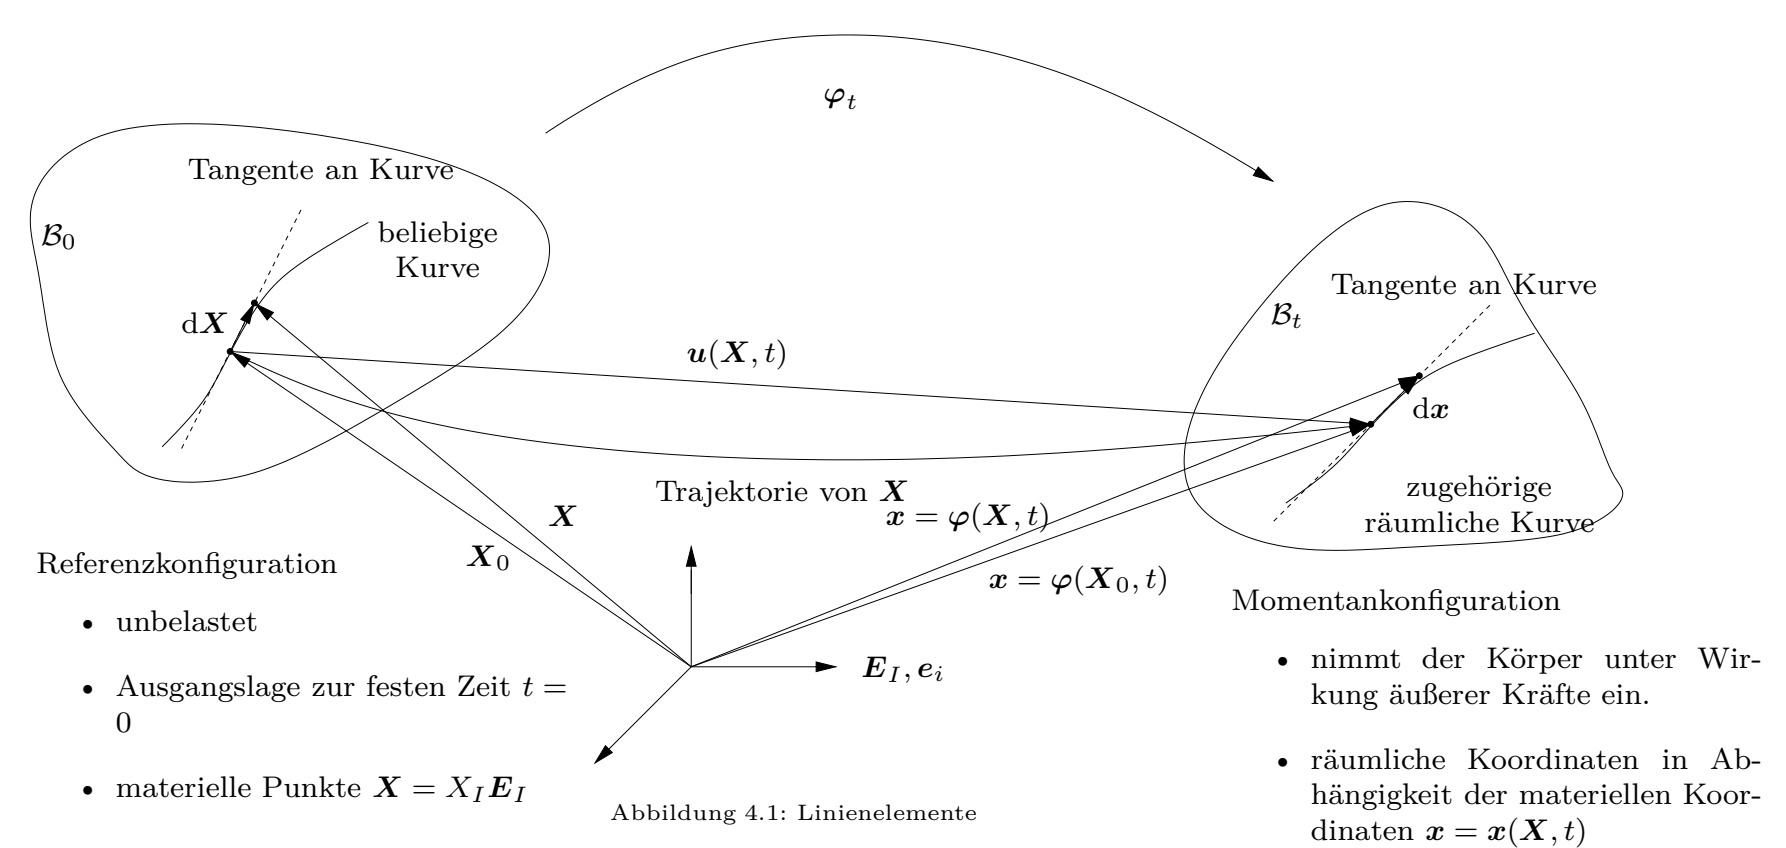
\includegraphics[width=0.7\textwidth]{Grafiken/Konfigurationsaenderung.jpg}
\subsection{Hyperelastisches Materialgesetz:}
        \includegraphics[width=0.45\textwidth]{Grafiken/Hyperelastizität.jpg}
\subsection{Massenbilanz:}
    \begin{itemize}
        \item Masse eines Körpers bleibt bei Deformation konstant
        \item Festkörpermechanik: $\rho_0 = \rho_t = konst.$
        \item Fluidmechanik: $div(v(\textbf{x},t))=0$
    \end{itemize} 
\subsection{Impulsbilanz} 
        \begin{itemize}
            \item Impuls eines Körpers ändert sich über die Zeit, durch am Körper angreifende Kräfte
            \item $\boldsymbol{\dot{P}}=\boldsymbol{F}^{ext}$
            \item $\rho_0 \boldsymbol{\dot{V}} = \rho_0 \boldsymbol{\Ddot{\varphi}} = \boldsymbol{B} + Div(\boldsymbol{P})$ oder $\rho_t \boldsymbol{\dot{v}} = \boldsymbol{b} + div\left(\boldsymbol{\sigma}^T\right)$
            \item $ \textbf{P} = \boldsymbol{v} \cdot m$
        \end{itemize}
\subsection{Drehimpulsbilanz} 
    \begin{itemize}
        \item Drehimpuls eines Körpers ändert sich über die Zeit, durch am Körper angreifende Momente
        \item $\boldsymbol{\dot{L}}=\boldsymbol{M}^{ext}$
        \item $0 (\text{Impulsbilanz}) =\boldsymbol{r} \times \left( \boldsymbol{\dot{V}} \rho_0 - \boldsymbol{B} - DIV\left(\boldsymbol{\Tilde{P}}^T\right) \right)$
        \item $\boldsymbol{r}=\boldsymbol{x-x}_0 \: (\text{räumlich}) = \boldsymbol{\varphi}(\boldsymbol{X},t) -\boldsymbol{x}_0 \: (\text{materiell}) $
    \end{itemize}
\subsection{Energiebilanz}
\begin{itemize}
    \item Die Gesamtenergie eines Körpers ändert sich durch die Leistung der über die Zeit angreifende Kräfte. Für konservative Systeme ist die Gesamtenergie konstant über die Zeit.
    \item Gesamtenergie: $E=T+U$
    \item Globale Form: $\dot{E}=\dot{T}+\dot{U} = P^{ext}$
    \item Lokale Form: $\dot{W}=\boldsymbol{P} : \boldsymbol{\dot{F}}$
    \item $T=$kinetische E. , $U=$innere E. , $u=$innere Energiedichte , $W =$ Verzerrungsenergiedichtefunktion
\end{itemize}
\subsection{Theoriewissen}
\begin{itemize}
    \item Cauchy zu Piola Spannungsvektor:\\
        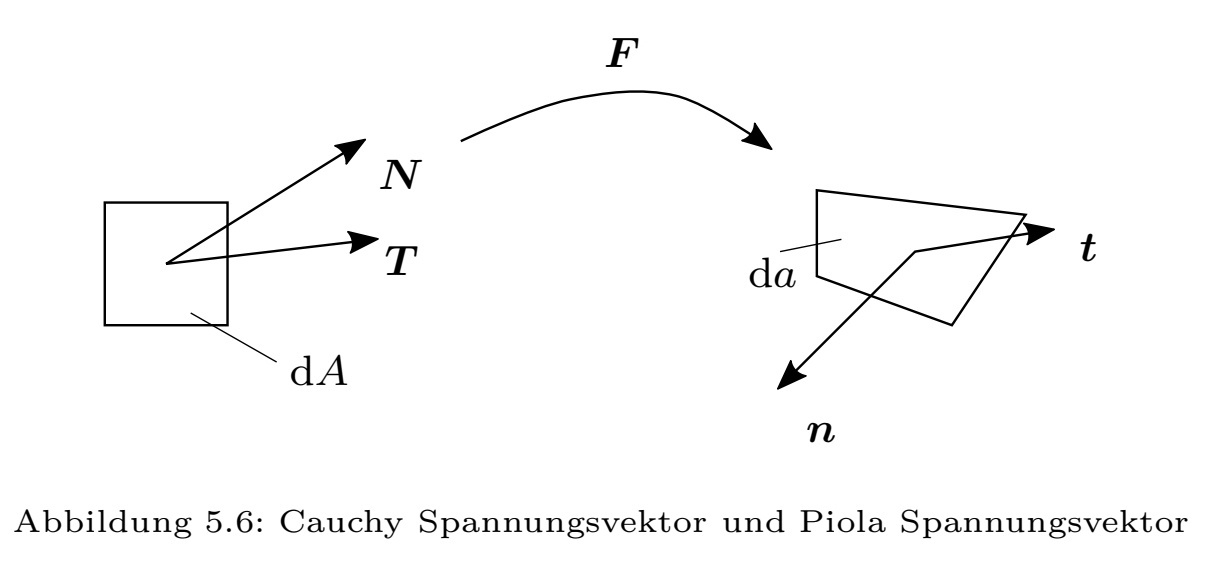
\includegraphics[width=0.45\textwidth]{Grafiken/Cauchy-Piola.jpg}
    \item Entropie: Möglichkeit eines Objekts verschiedene Zustände anzunehmen
    \item Wann existiert Hyperelastizität?:
        \begin{itemize}
            \item wenn ideale Verzerrungsenergiedichte existiert: $\underline{P}=\frac{\delta W (\underline{F})}{\delta \underline{F}}$
            \item anhängig vom aktuellen Deformationszustand
        \end{itemize}
    \item Lineare/nichtlineare Probleme: Lineare Probleme nur auf kleine Deformationen anwendbar
\end{itemize}

\newpage
\section{Anfangsrandwertprobleme}
\includegraphics[page=1]{Grafiken/ARWP1.pdf}
\newpage
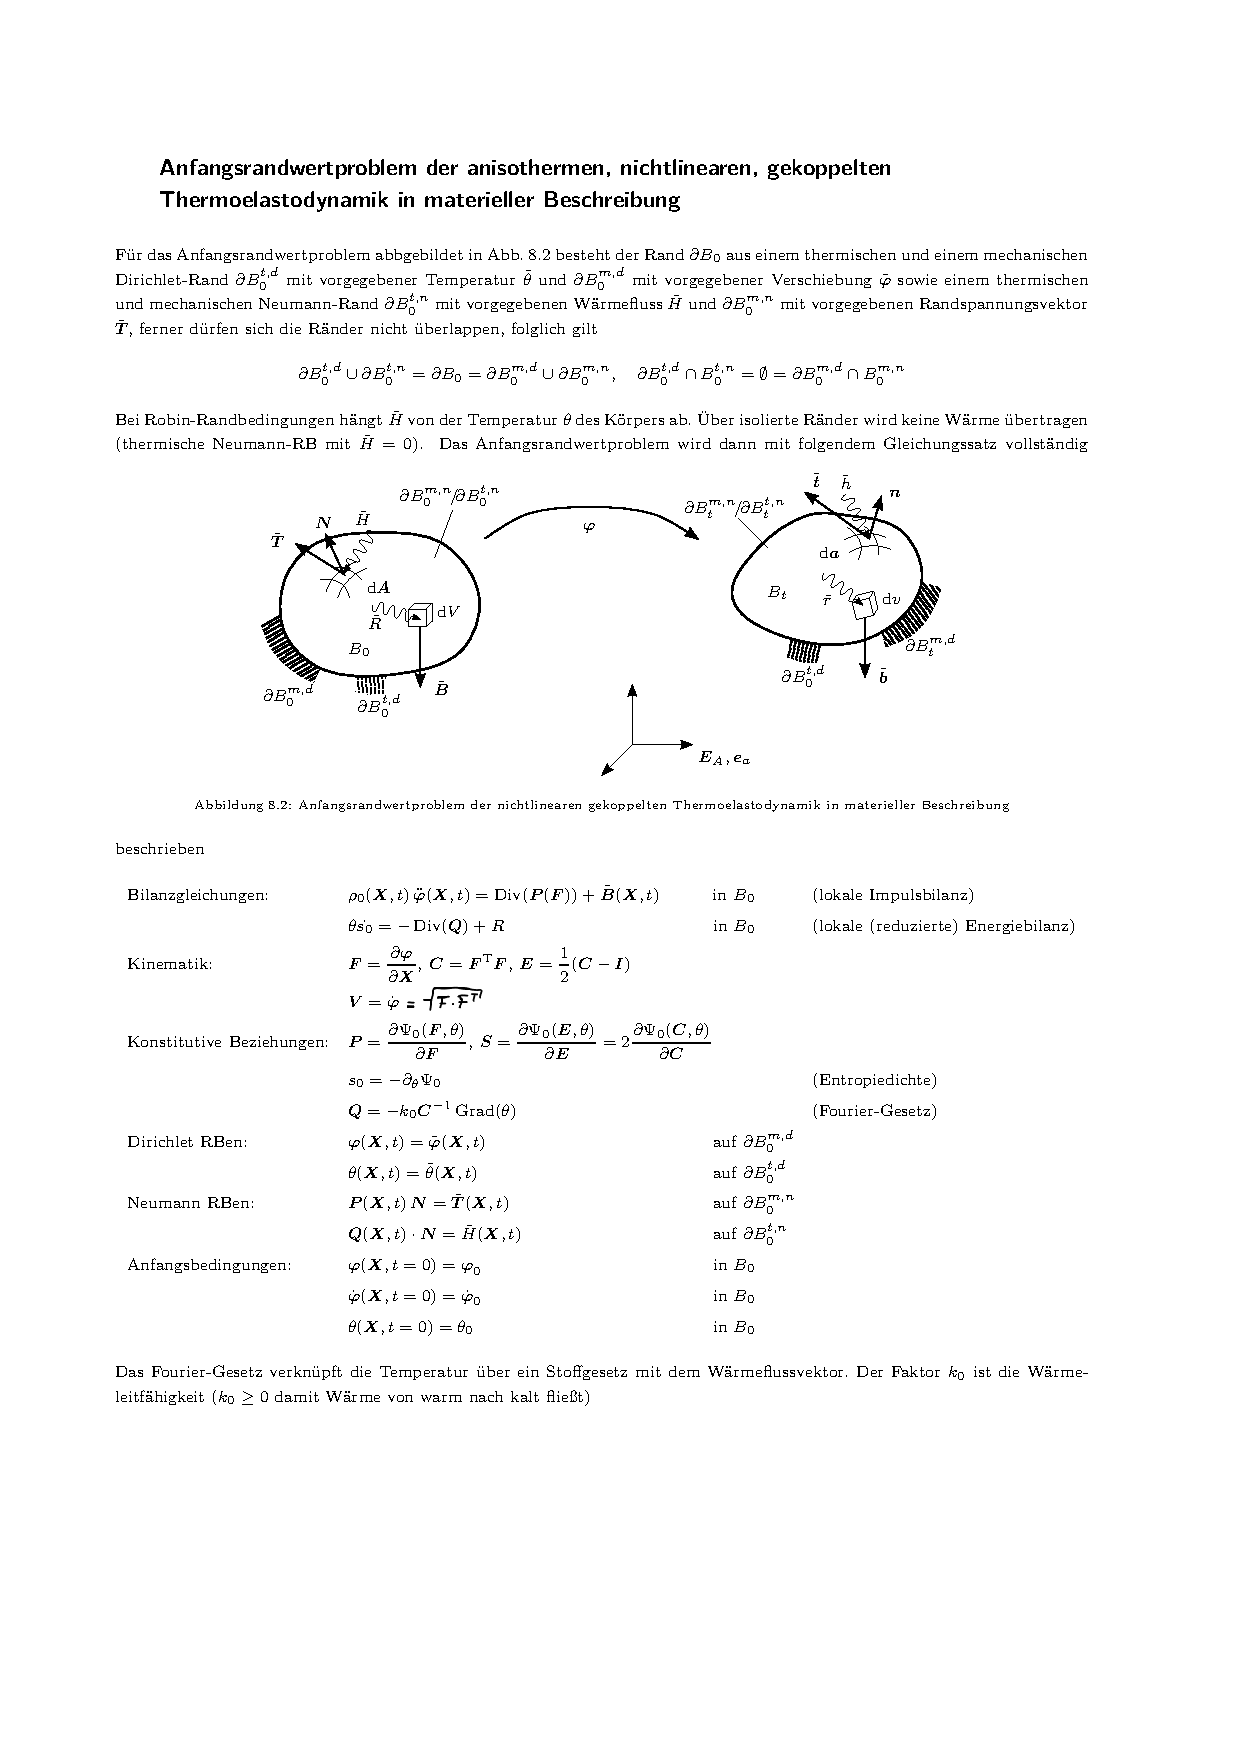
\includegraphics[page=1]{Grafiken/ARWP2.pdf}
\newpage

\section{Theoriefragen}

\end{document}
















